\chapter{INTRODUCTION}

\section{Background to the study}
 [Background to the study detail]

\section{Problem Statement}
 [Problem statement detail]

Figure~\ref{fig:example_fig} shows an example figure.

\begin{figure}[h!]
    \centering
    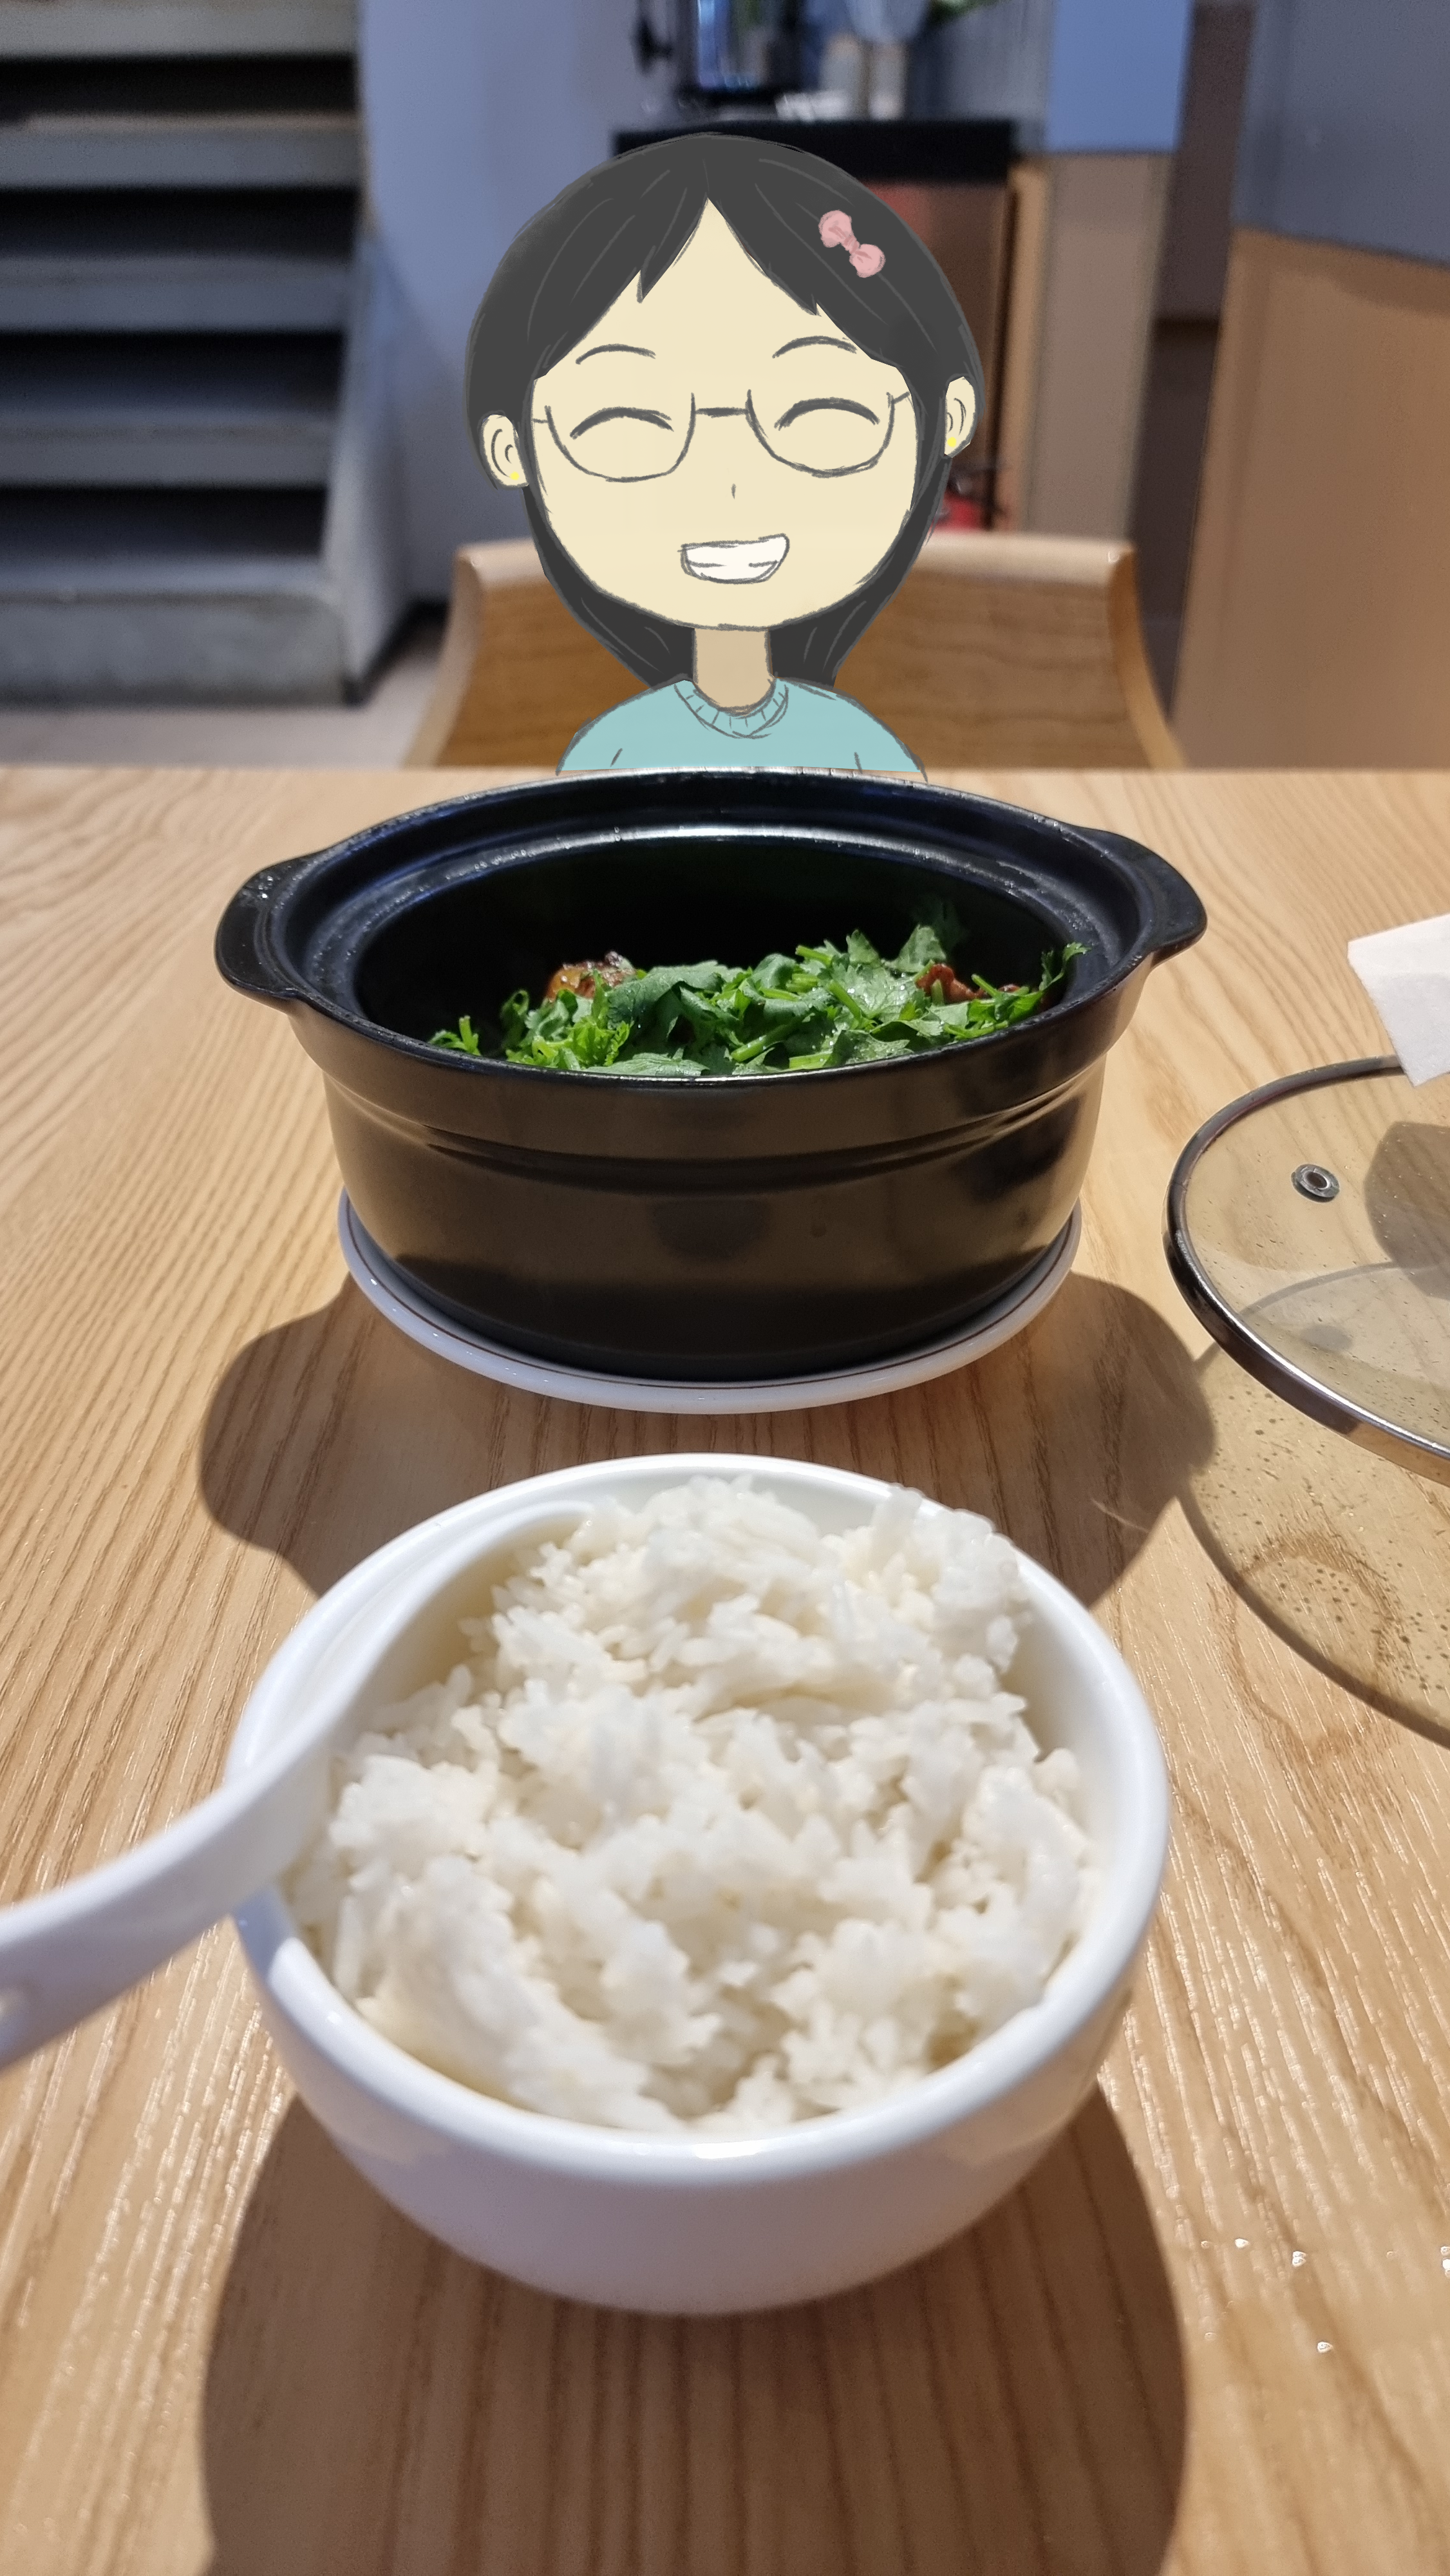
\includegraphics[width=0.5\textwidth]{figures/example.png}
    \caption{Example figure}
    \label{fig:example_fig}
\end{figure}

\subsection{Subsection}
[Subsection detail]

Table~\ref{tab:example_tab} shows an example table.
\begin{table}[h]
    \centering
    \caption{Example table}
    \label{tab:example_tab}
    \begin{tabularx}{\textwidth}{|X|X|X|}
        \hline
        \textbf{Column 1} & \textbf{Column 2} & \textbf{Column 3} \\
        \hline
        Data 1            & Data 2            & Data 3            \\
        \hline
        Data 4            & Data 5            & Data 6            \\
        \hline
        Data 7            & Data 8            & Data 9            \\
        \hline
    \end{tabularx}
\end{table}